
% !TeX spellcheck = pt_BR
% !TEX encoding = UTF-8 Unicode

\chapter{Exponencial e logaritmo}\label{CAP:ExponLog}

\ifdefined\updateans
% Only need to run once in a lifetime, when the file ans.tex needs to be updated.
\Writetofile{ans}{\protect\section*{Capítulo \ref{CAP:ExponLog}}}
\fi

%\citacao{$S=k_B\log W$}{L. Boltzmann}

O objetivo nesse capítulo é definir e descrever as principais
propriedades de uma das funções mais importantes da matemática, a
\grasA{exponencial de base $a$},\index{função!
exponencial}\index{exponencial! na base $e$} 
%\inputimage
e da sua função inversa, o \grasA{logaritmo na base $a$},\index{função!
logaritmo}\index{logaritmo! na base $a$}
%inputimage

Os exemplos de uso dessas duas funções em ciências são inúmeros. Vejamos dois
exemplos onde elas aparecem nos axiomas de uma teoria:

\begin{ex}\label{Ex:Fisstat}\index{física estatística}
Em \emph{física estatística}, estudam-se sistemas em equilíbrio termodinâmico. 
Suponha que um sistema pode estar, no equilíbrio, em 
um dos $N$ microestados $x_1,\dots,x_N$ de energias respectivas $E_1,\dots,E_N$.
Se a temperatura é $T$, a \grasA{probabilidade do sistema estar no estado $i$} é
dada por 
$$p_i=\frac{e^{-\tfrac{E_i}{k_BT}}}{Z}\,,$$
onde $e^x$ é a função exponencial na base $e=2.718...$ (ver Seção
\ref{Sec:ExpoLog}), $k_B$ é a \grasA{constante de Boltzmann} e $Z$ a
\grasA{função de partição}.
\end{ex}

\begin{ex}
Em \emph{Teoria da Informação,}\index{informação! teoria da} estudam-se sequências
infinitas de símbolos
aleatórios. Com um alfabeto binário $\bA=\{0,1\}$,
$$01101001000011011011001001101010011001000000111010101100110....$$
Com um alfabeto $\bA=\{0,1,2,\dots,8,9\}$,
$$43895612031468275092781059463897360142581974603522706194583...$$
Se cada algarismo $a_i$ de um alfabeto 
$\bA=\{a_1,a_2,\dots,a_k\}$ aparece com uma probabilidade $p_i$, onde
$\sum_{j=1}^kp_j=1$, então a \grasA{Entropia de Shannon} de uma sequência
aleatória com essa propriedade é definida por
$$S=-\sum_{j=1}^kp_j\log_2 p_j\,,$$
onde o logaritmo é na base $2$ (mas pode ser tomado numa base qualquer).
$S$ dá um limite para a maior \grasA{taxa de compactação} para essa sequência.
\end{ex}

Uma construção completa das funções $\exp_ax$, $\log_a x$, para todo $x\in \bR$,
como se encontra nos livros de análise, requer um conhecimento detalhado das
propriedades dos números reais. Aqui daremos uma construção que, apesar de não
ser completamente rigorosa, tem a vantagem de ser intuitiva (espera-se) e permitirá
usar essas funções já desde o próximo capítulo.

\section{Exponencial}\label{Sec:Exponencial}

Seja $a>0$ um número positivo, fixo, chamado \grasA{base}. Definamos primeiro,
para todo número natural $n\in\bN$,
$$\exp_a(n)\pardef a^n= a\cdot a\cdots a\,\quad \text{($n$ vezes)}\,.$$
(Em particular, $a^1=a$.)
Assim obtemos uma função
\begin{align*}
 \exp_a:\bN&\to (0,\infty)\\
n&\mapsto a^n\,,
\end{align*}
que satisfaz às seguintes propriedades: para todo $m,n\in\bN$,
\begin{align}
a^ma^n&=a^{m+n}\,,\label{Eq:Proprexp1}\\
(a^m)^n&=a^{m\cdot n}\,.\label{Eq:Proprexp2}
\end{align}
Se $b>0$ for uma outra base,
\begin{equation}
(a\cdot b)^n=a^nb^n\,.\label{Eq:Proprexp3}
\end{equation}

O nosso objetivo é de estender essa função à reta real toda:
\begin{align*}
 \exp_a:\bR&\to (0,\infty)\\
x&\mapsto a^x\,.
\end{align*}
Faremos essa extensão passo a passo, com o seguinte objetivo em mente: \emph{que
as relações \eqref{Eq:Proprexp1}-\eqref{Eq:Proprexp3} sejam sempre satisfeitas,
também para variáveis reais.}\\

Por exemplo, como definir $a^0$? Para \eqref{Eq:Proprexp1} ser satisfeita com
$m=0$, $n=1$,
$$a=a^1=a^{1+0}=a^1\cdot a^0=a\cdot a^0\,.$$
Daí, simplificando por $a$ na última expressão, 
vemos que é preciso definir $$a^0\pardef 1\,.$$ 
Podemos em seguida definir a exponencial dos inteiros {negativos}, $a^{-n}$.
Usando de novo \eqref{Eq:Proprexp1} com $m=-n$, temos
$$a^{n}a^{-n}=a^{n-n}=a^0=1\,.$$
Logo, vemos que $a^{-n}$ precisa ser definida como:
$$
a^{-n}\pardef \frac{1}{a^n}\,.
$$
O mesmo raciocínio pode ser aplicado em geral: se $a^x$ já foi definido para
$x>0$, então o único jeito de definir $a^{-x}$ é como: 
$$a^{-x}\pardef \tfrac{1}{a^x}\,.$$ 
Estamos por enquanto com uma função 
\begin{align*}
 \exp_a:\bZ&\to (0,\infty)\\
n&\mapsto a^n\,.
\end{align*}
Façamos um primeiro esboço, isto é,
representemos alguns pontos de coordenadas $(n,a^n)$, $n\in \bZ$, no plano
cartesiano
(nessa figura, $a=2$):
\begin{center}
\begin{bmlimage}\begin{tikzpicture}[scale=0.8]
\begin{scope}
\draw[->] (-4,0)--(2.5,0) node[right]{$\bZ$};
\draw[->] (0,-0.2)--(0,5) node[left]{$a^n$};
\draw[color=gray!30, domain=-4:2.1]  plot (\x,{exp(\x*ln(2)}) node[right]{$a^x$};
\draw (0,1) node[left]{$1$};
\foreach \k in {-4,...,2} {
\pgfmathsetmacro{\y}{2^(\k)};
\fill (\k,\y) circle (0.45mm);
\draw (\k,0) node{$\shortmid$};
\draw (\k,0) node[below]{$\k$};
\draw[dotted] (\k,0)--(\k,\y);
}
\end{scope}
\end{tikzpicture}\end{bmlimage}
\end{center}
Já podemos observar que para valores de $n$ positivos grandes (aqui $a=2$), 
$$2^1=2\,\quad 2^2=4\,,\quad 2^3=8\,\quad 2^4=16\,,\quad 2^5=32\,,\quad
2^6=64\,,...$$
Como cada elemento dessa sequência é o \emph{dobro} do anterior, ela
\emph{diverge exponencialmente}\index{exponencial! divergência} rápido.
Por outro lado, para valores de $n$ negativos grandes, a sequência
\emph{converge exponencialmente} rápido para zero: 
$$
2^{-1}=0.5\,,\quad 2^{-2}=0.25\,,\quad 2^{-3}=0.125\,,\quad
2^{-4}=0.0625\,,\quad 2^{-5}=0.03125\,...
$$

Agora que $a^x$ foi definida para os valores de $x$ inteiros, vejamos como 
definir $a^x$ para os semi-inteiros
$x\in\{\dots,-\frac52,-\frac32,-\frac12, \frac12, \frac32,\frac52,\dots\}$.
Por exemplo, se $x=\tfrac{1}{2}$, já que $(a^{\frac12})^2=a$ por
\eqref{Eq:Proprexp2}, vemos que
$a^{\frac12}=\sqrt{a}$. Para definir $a^x$ para $x=\frac{m}{2}$, $m\in\bZ$,
usemos também \eqref{Eq:Proprexp2}. Quando $m>0$,
$$
a^{\frac{m}{2}}\pardef (a^{\frac{1}{2}})^m=\sqrt{a}^m\,,$$
e quando $m<0$,
$$\quad a^{-\frac{m}{2}}\pardef \frac{1}{a^{\frac{m}{2}}}\,.
$$
Assim, o gráfico anterior pode ser acrescentado dos pontos da forma
$(\tfrac{m}{2},a^{\frac{m}{2}})$:

\begin{center}
\begin{bmlimage}\begin{tikzpicture}[scale=0.8]
\begin{scope}
\draw[->] (-4,0)--(2.5,0);
\draw[->] (0,-0.2)--(0,5);
\draw[color=gray!30, domain=-4:2.1]  plot (\x,{exp(\x*ln(2))}) node[right]{$a^x$};
\foreach \k in {-8,...,4} {
\pgfmathsetmacro{\y}{exp(\k*ln(2)/2)};
\fill (\k/2,\y) circle (0.45mm);
}
\foreach \k in {-4,...,2} {
\draw (\k,0) node{$\shortmid$};
\draw (\k,0) node[below]{$\scriptstyle{\k}$};
\pgfmathsetmacro{\y}{exp(\k*ln(2))};
\draw[dotted] (\k,0)--(\k,\y);
}
\foreach \k in {-7,-5,-3,-1,1,3} {
\draw (\k/2,0) node{$\shortmid$};
%\draw (\k/2,-0.1) node[below]{$\scriptscriptstyle{\tfrac{\k}{2}}$};
}
\end{scope}
\end{tikzpicture}\end{bmlimage}
\end{center}

Repetindo esse processo, $a^x$ pode ser definido para os pontos da forma
$\tfrac{m}{4}$, $\tfrac{m}{8}$, $\tfrac{m}{16}$, etc, obtendo assim uma função
definida para qualquer $x$ da forma $\tfrac{m}{2^k}$. Esses reais são chamados
de \grasA{racionais diádicos}.

\begin{center}
\begin{bmlimage}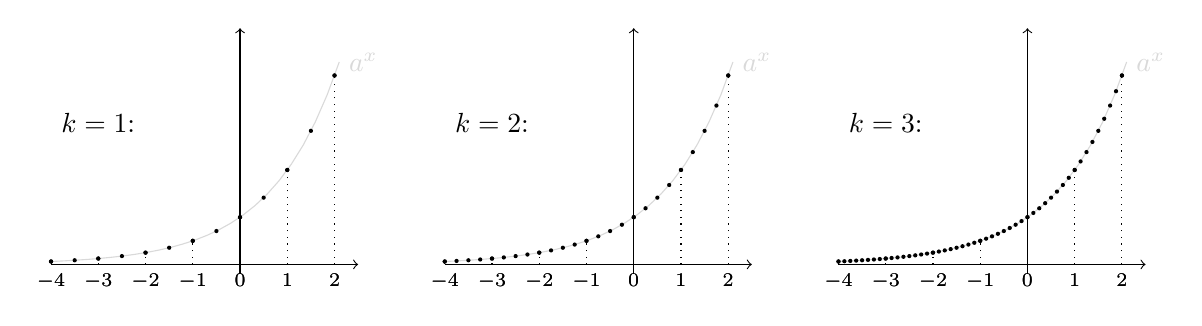
\begin{tikzpicture}
\begin{scope}[scale=0.6]
\draw[->] (-4,0)--(2.5,0);
\draw[->] (0,-0.2)--(0,5);
\draw[color=gray!30, domain=-4:2.1] plot (\x,{exp(\x*ln(2))}) node[right]{$a^x$};
\foreach \k in {-4,...,2} {
\draw (\k,0) node{$\shortmid$};
\draw (\k,0) node[below]{$\scriptstyle{\k}$};
\pgfmathsetmacro{\y}{2^(\k)};
\fill (\k,\y) circle (0.45mm);
\draw[dotted] (\k,0)--(\k,\y);
}
\foreach \i in {-4,...,2} {
\draw (\i,0) node[below]{$\scriptstyle{\i}$};
}
%%%%%%%%%%%
\draw (-3,3) node{$k=1$:};
\pgfmathsetmacro{\l}{2};
\pgfmathsetmacro{\n}{6*\l};
\foreach \k in {0,...,\n} {
\pgfmathsetmacro{\x}{-4+\k/\l};
\pgfmathsetmacro{\y}{exp(\x*ln(2))};
\draw (\x,0) node{$\shortmid$};
\fill (\x,\y) circle (0.45mm);
}
\end{scope}
\begin{scope}[xshift=5cm, scale=0.6]
\draw[->] (-4,0)--(2.5,0);
\draw[->] (0,-0.2)--(0,5);
\draw[color=gray!30, domain=-4:2.1]  plot (\x,{exp(\x*ln(2))}) node[right]{$a^x$};
\foreach \k in {-4,...,2} {
\draw (\k,0) node{$\shortmid$};
\draw (\k,0) node[below]{$\scriptstyle{\k}$};
\pgfmathsetmacro{\y}{2^(\k)};
\fill (\k,\y) circle (0.45mm);
\draw[dotted] (\k,0)--(\k,\y);
}
\foreach \i in {-4,...,2} {
\draw (\i,0) node[below]{$\scriptstyle{\i}$};
}
%%%%%%%%%%%
\draw (-3,3) node{$k=2$:};
\pgfmathsetmacro{\l}{4};
\pgfmathsetmacro{\n}{6*\l};
\foreach \k in {0,...,\n} {
\pgfmathsetmacro{\x}{-4+\k/\l};
\pgfmathsetmacro{\y}{exp(\x*ln(2))};
\draw (\x,0) node{$\shortmid$};
\fill (\x,\y) circle (0.45mm);
}
\end{scope}

\begin{scope}[xshift=10cm, scale=0.6]
\draw[->] (-4,0)--(2.5,0);
\draw[->] (0,-0.2)--(0,5);
\draw[color=gray!30, domain=-4:2.1]  plot (\x,{exp(\x*ln(2))}) node[right]{$a^x$};
\foreach \k in {-4,...,2} {
\draw (\k,0) node{$\shortmid$};
\draw (\k,0) node[below]{$\scriptstyle{\k}$};
\pgfmathsetmacro{\y}{2^(\k)};
\fill (\k,\y) circle (0.45mm);
\draw[dotted] (\k,0)--(\k,\y);
}
\foreach \i in {-4,...,2} {
\draw (\i,0) node[below]{$\scriptstyle{\i}$};
}
%%%%%%%%%%%
\draw (-3,3) node{$k=3$:};
\pgfmathsetmacro{\l}{8};
\pgfmathsetmacro{\n}{6*\l};
\foreach \k in {0,...,\n} {
\pgfmathsetmacro{\x}{-4+\k/\l};
\pgfmathsetmacro{\y}{exp(\x*ln(2))};
\draw (\x,0) node{$\shortmid$};
\fill (\x,\y) circle (0.45mm);
}
\end{scope}

\end{tikzpicture}\end{bmlimage}
\end{center}

Observe que a medida que $k$ aumenta, 
os racionais diádicos $\tfrac{m}{2^k}$\index{números! racionais diádicos} vão enchendo a
reta real: diz-se que eles
formam um conjunto \emph{denso}\index{conjunto! denso} na reta.\\

Mas todos os racionais diádicos são racionais, e existem muitos (!) reais que
não são racionais...
Daremos a idéia da última (e mais delicada) etapa da construção de $a^x$ para
qualquer real $x$. Procederemos por \emph{aproximação}, observando que
qualquer real $x$ pode ser cercado por dois diádicos, digamos $z_-$ e $z_+$,
arbitrariamente próximos um do outro.
\begin{ex}
Por exemplo, $\pi=3.141592\dots$ é irracional~\footnote{A irracionalidade de
$\pi$ foi provada pela primeira vez por Johann Heinrich Lambert em $1761$.}, 
e é possível obter
aproximações pegando sucessivamente diádicos com $k=0,1,2,\dots$,etc.:
\begin{align*}
3=\frac{3}{2^0}& <\pi < \frac{4}{2^0}=4\\
3=\frac{6}{2^1}& <\pi < \frac{7}{2^1}=3.5\\
3=\frac{12}{2^2}& <\pi < \frac{13}{2^2}=3.250\\
3.125=\frac{25}{2^3}& <\pi < \frac{26}{2^3}=3.250\,\quad \text{etc.}
\end{align*}
Assim, podemos sempre achar um diádico, ou maior ou menor do que $\pi$, cujo valor
numérico é arbitrariamente perto de $\pi$.
\end{ex}

Assim, para qualquer irracional $x$, é possível escolher uma
sequência decrescente de diádicos $z_n^+$ que \emph{tende a $x$}, 
$z_n^+\searrow x$, e uma sequência crescente de diádicos $z_n^-$ 
\emph{que tende a $x$}, $z_n^-\nearrow x$. 

\begin{center}
\begin{bmlimage}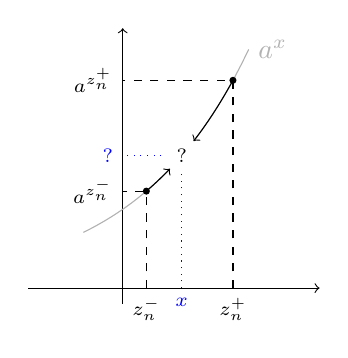
\begin{tikzpicture}
 \draw[ ->] (-1.2,0)--(2.5,0);
\draw[->] (0,-0.2)--(0,3.3);
\draw[color=gray!60, domain=-0.5:1.6]  plot (\x,{exp(\x*ln(2))}) node[right]{$a^x$};
\pgfmathsetmacro{\x}{0.75};
\draw[dotted, color=blue!100] (\x,0)
node[below]{$\scriptstyle{x}$}--(\x,{exp(\x*ln(2))})--(0,{exp(\x*ln(2))})
node[left]{$\scriptstyle{?}$};
\draw (\x,{exp(\x*ln(2))}) node[fill=white]{$\scriptstyle{?}$};
\pgfmathsetmacro{\x}{0.3};
\draw[->, domain=\x:\x+0.3]  plot (\x,{exp(\x*ln(2))});
\draw[dashed] (\x,0) node[below]{$\scriptstyle{z_n^-}$}--(\x,{exp(\x*ln(2))})--(0,{exp(\x*ln(2))})
node[left]{$\scriptstyle{a^{z_n^-}}$};
\fill (\x, {exp(\x*ln(2))}) circle (0.45mm);
\pgfmathsetmacro{\x}{1.4};
\draw[<-, domain=\x-0.5:\x]  plot (\x,{exp(\x*ln(2))});
\fill (\x, {exp(\x*ln(2))}) circle (0.45mm);
\draw[dashed] (\x,0)
node[below]{$\scriptstyle{z_n^+}$}--(\x,{exp(\x*ln(2))})--(0,{exp(\x*ln(2))})
node[left]{$\scriptstyle{a^{z_n^+}}$};
\end{tikzpicture}\end{bmlimage}
\end{center}
Vemos então que os valores de $a^{z_n^-}$ e $a^{z_n^+}$ se aproximam de um
valor comum, que será usado para definir o valor de $a^x$.

Observe que essa construção usa implicitamente, pela primeira vez, a idéia
sutil de \emph{limite}\index{limite}, que será apresentada no próximo capítulo: qualquer
real
$x$ pode ser \emph{aproximado por uma sequência}\index{aproximação! por racionais} $z_n$
de racionais diádicos: 
$$x=\lim_{n\to \infty}z_n\,.$$ 
Como $a^{z_n}$ já foi definida para cada $z_n$ da sequência, $a^x$ é definida como 
$$a^x\pardef \lim_{n\to \infty}a^{z_n}\,.$$
Pode ser mostrado que a função $x\mapsto a^x$ obtida satisfaz às propriedades
\eqref{Eq:Proprexp1}-\eqref{Eq:Proprexp3}. Por exemplo, se $y$ é um outro real,
aproximado pela sequência $w_n$, $y=\lim_{n\to \infty}w_n$, então $x+y$ pode ser
aproximado pela sequência $(z_n+w_n)$, logo
$$
a^{x+y}=\lim_{n\to \infty}a^{z_n+w_n}
=\lim_{n\to \infty}a^{z_n}a^{w_n}
=(\lim_{n\to \infty}a^{z_n})(\lim_{n\to \infty}a^{w_n})=a^xa^y\,.
$$
Todas as operações acima são corretas, mas precisam ser justificadas.

AQUI
Assim conseguimos definir a função \grasA{exponencial  na base $a>0$}\index{exponencial!
na base $a$|textbf} como uma
função definida na reta real inteira:
\begin{align*}
 \exp_a:\bR&\to(0,\infty)\\
x&\mapsto a^x\,.
\end{align*}
Ela foi construida de maneira tal que as seguintes propriedades sejam
satisfeitas: $a^0=1$,\index{exponencial! propriedades}
\begin{align}
a^xa^y&=a^{x+y}\label{Eq:PropExpon1}\\
(a^x)^y&=a^{xy}\label{Eq:PropExpon2}\\
\frac{a^x}{a^y}&=a^{x-y}\label{Eq:PropExpon3}\\
(ab)^x&=a^xb^x\label{Eq:PropExpon4}\,.
\end{align}
Todas as funções exponenciais com base $a>1$ têm gráficos parecidos: 

\begin{center}
\begin{bmlimage}\begin{tikzpicture}\label{Fig:graficosdifbases}
\begin{scope}[scale=0.8]
\draw[->] (-4,0)--(2.5,0) node[right]{$x$};
\draw[->] (0,-0.2)--(0,5) node[left]{$a^x$};
\draw[domain=-4:2.1]  plot (\x,{exp(\x*ln(2))}) node[right]{$a=2$};
\draw[dashed, domain=-4:2.1]  plot (\x,{exp(\x*ln(1.5))}) node[right]{$a=\tfrac32$};
\draw[dotted, domain=-4:1.5]  plot (\x,{exp(\x*ln(3))}) node[right]{$a=3$};
\foreach \k in {-4,...,2} {
\draw (\k,0) node{$\shortmid$};
\draw (\k,0) node[below]{$\scriptstyle{\k}$};
}
\end{scope}
\end{tikzpicture}\end{bmlimage}
\end{center}
Observe que todos os gráficos passam pelo ponto $(0,1)$, e que $x\mapsto a^x$
é \emph{estritamente crescente}:
$$x<y\quad \Leftrightarrow \quad a^x<a^y\,.$$


Para os valores $a<1$, basta usar uma simetria:
Para $a=\frac12$ por exemplo, podemos observar que 
$$\exp_{{\frac12}}(x)=(\tfrac12)^x=2^{-x}=\exp_2(-x)\,.$$
Portanto, o gráfico de $x\mapsto (\frac12)^x$ é obtido a partir do gráfico de
$x\mapsto 2^x$ por uma simetria pelo eixo $y$. Em geral, o gráfico de $x\mapsto
(\frac1a)^x$ é obtido a partir do gráfico de $x\mapsto a^x$ por uma simetria
pelo eixo $y$:
\begin{center}
\begin{bmlimage}\begin{tikzpicture}
\begin{scope}[scale=0.8]
\draw[->] (-2.5,0)--(4.3,0) node[right]{$x$};
\draw[->] (0,-0.2)--(0,5) node[right]{$a^x$};
\draw[domain=-4:2.1]  plot (-\x,{exp(\x*ln(2))}) node[left]{$a=\tfrac12$};
\draw[dashed, domain=-4:2.1]  plot (-\x,{exp(\x*ln(1.5))}) node[left]{$a=\tfrac23$};
\draw[dotted, domain=-4:1.5]  plot (-\x,{exp(\x*ln(3))}) node[left]{$a=\tfrac13$};
\foreach \k in {-2,...,4} {
\draw (\k,0) node{$\shortmid$};
\draw (\k,0) node[below]{$\scriptstyle{\k}$};
}
\end{scope}
\end{tikzpicture}\end{bmlimage}
\end{center}
Temos também que  quando $0<a<1$, $x\mapsto a^x$ 
é \emph{estritamente decrescente}:
$$x<y \quad \Leftrightarrow \quad  a^x>a^y\,.$$

\begin{exo}
Esboce os gráficos das funções $1-2^{-x}$, $3^{x-1}$, $(\tfrac32)^{-x}$,
$-(\frac32)^{|x|}$.
\begin{sol} Todos os gráficos podem ser obtidos por transformações de
$2^x$,\index{gráfico! transformação de}
$3^x$ e $(\frac32)^x$:
\begin{center}
 \begin{bmlimage}\begin{tikzpicture}[scale=0.7]
\draw[->] (-4.5,0)--(4.3,0) node[right]{$x$};
\draw[->] (0,-3)--(0,5);
\draw[domain=-2.1:4.1]  plot (\x,{1-exp(-\x*ln(2))}) node[right]{$1-2^{-x}$};
\draw[domain=-3.4:2.5]  plot (\x,{exp((\x-1)*ln(3))}) node[above]{$3^{x-1}$};
\draw[domain=-3.7:2.4]  plot (-\x,{exp(\x*ln(1.5)))})
node[above]{$(\tfrac{3}{2})^{-x}$};
\draw[domain=-3:3]  plot (\x,{(-1)*(exp(abs(\x)*ln(1.5)))})
node[right]{$-(\tfrac{3}{2})^{|x|}$};
\draw[dotted] (-3,1)--(4,1);
\draw (0,1) node[above right]{$1$};
 \end{tikzpicture}\end{bmlimage}
\end{center}
\end{sol}
\end{exo}

Com mais funções, resolvem-se mais (in)equações:
\begin{ex}
Resolvamos $$3^x+3^{-x}=2\,.$$
Multiplicando por $3^x$ em ambos lados e agrupando os termos obtemos
$(3^x)^2-2\cdot 3^x+1=0$. Chamando $z=3^x$, essa equação se torna $z^2-2z+1=0$,
cuja única solução é $z=1$, isto é, $3^x=1$. Logo, $S=\{0\}$.
\end{ex}

\begin{exo}
Resolva:
\begin{multicols}{3}
 \begin{enumerate}
  \item\label{itexoresolexp1} $5^x+25\cdot 5^{-x}=26$
  \item\label{itexoresolexp2} $(2^x)^2=16$
  \item\label{itexoresolexp3} $2^{x+1}-16\leq 0$
  \item\label{itexoresolexp6} $3^x>\tfrac19$
 \item\label{itexoresolexp4} $(2^x-2)(\tfrac{1}{5^x}-1)<0$
 \item\label{itexoresolexp5} $2^{2x+1}\geq 5^{1-x}$
 \end{enumerate}
\end{multicols}
\vspace{0.01cm}
\begin{sol}
\eqref{itexoresolexp1} $S=\{0,2\}$.
\eqref{itexoresolexp2}  Tomando a raiz: $2^x=\pm 4$, mas como a função
exponencial somente toma valores positivos, $2^x=-4$ não possui soluções. Logo,
$S=\{2\}$.
\eqref{itexoresolexp3} Escrevendo a inequação como $2^{x+1}\leq 2^4$, vemos que
$S=\{x:x+1\leq 4\}=(-\infty,3]$.
\eqref{itexoresolexp6} $S=(-2,\infty)$.
\eqref{itexoresolexp4} $S=(-\infty,0)\cup (1,\infty)$.
\eqref{itexoresolexp5} $S=(\log_{20}\tfrac52,\infty)$.
\end{sol}
\end{exo}

\begin{obs}
Para se acostumar com a as mudanças de escala entre os valores de $10^{n}$ para
$n$ grande positivo e $n$ grande negativo, sugiro assistir o pequeno filme
clássico de Charles e Bernice Ray Eames de $1968$: \emph{Powers of Ten}
(\emph{Potências de dez})\index{potência! Potências de dez (filme)}. Se encontra por
exemplo em:
\verb|http://www.youtube.com/watch?v=0fKBhvDjuy0|.
\end{obs}

\begin{obs}
Lembramos que a base de uma exponencial é sempre \emph{estritamente positiva}.
De fato, definir a exponencial para bases negativas, por exemplo $a=-1$, daria 
problemas já para definir $(-1)^{1/2}$, que corresponde a $\sqrt{-1}$, que
não é definido nos reais.
Observe também que a base $a=0$ não é interessante, mas mesmo assim daremos um 
sentido a ``$0^0$'' no Capítulo~\ref{Cap:Derivacao}.
\end{obs}

\section{Logaritmo}\index{logaritmo|textbf}
Como a exponencial $x\mapsto \exp_ax$ é estritamente crescente (ou decrescente
se $0<a<1$), é uma bijeção de $\bR$ para $(0,\infty)$, e
a sua função inversa é bem definida, chamada \grasA{logaritmo na base $a$}:
\begin{align*}
\log_a:(0,\infty)&\to \bR \\
y&\mapsto \log_ay\,.
\end{align*}
Como $a^0=1$, temos $\log_a1=0$, e como $a^1=a$ temos $\log_aa=1$.  
O gráfico do logaritmo, dependendo da base, é da forma\index{logaritmo! gráfico}:
\begin{center}
\begin{bmlimage}\begin{tikzpicture}[scale=0.7]
\begin{scope}
\draw (-1,3) node[left]{$a>1:$};
\draw[->] (-0.2,0)--(4,0) node[right]{$x$};
\draw[->] (0,-3)--(0,3) node[left]{$y$};
\draw (1,0) node{$\shortmid$} node[above]{$1$};
\draw[thick, domain=-3:1.7]  plot ({exp(\x)},\x) node[right]{$\log_ax$};
\draw[dotted] (2.718,0) node[below]{$a$}--(2.718,1)--(0,1) node[left]{$1$}
node{$-$};
\end{scope}
\begin{scope}[xshift=12cm]
\draw (-1,3) node[left]{$0<a<1:$};
\draw[->] (-0.2,0)--(4,0) node[right]{$x$};
\draw[->] (0,-3)--(0,3) node[left]{$y$};
\draw (1,0) node{$\shortmid$} node[above]{$1$};
\draw[thick, domain=-3:1.7]  plot ({exp(\x)},-\x) node[right]{$\log_ax$};
\end{scope}
\end{tikzpicture}\end{bmlimage}
\end{center}
O logaritmo é estritamente crescente se $a>1$, estritamente decrescente se
$0<a<1$.
Por definição,
\eq{
\label{eq_ExpLog_debase}
\forall x>0\,:\, a^{\log_ax}=x\,,\quad \text{ e } \forall x\in
\bR\,:\,\log_a(a^x)=x\,.}

A definição do logaritmo deve ser lembrada pela seguinte equivalência:
\eq{
z=\log_ax\quad\Leftrightarrow\quad a^z=x\,.
}
Por exemplo, para calcular $\log_28$, basta chamar $z=\log_28$, que é
equivalente a 
$2^z=8$, cuja única solução é $z=3$.

\begin{obs}
O logaritmo foi inventado por Napier~\footnote{John Napier, Merchiston (Escócia)
1550 - 1617.}\index{Napier, John} no século $XVI$, numa época em que ainda não existiam
calculadoras. 
Suponha que se queira calcular, \emph{na mão}, uma potência de um número grande.
Por exemplo: $9846^6$. A conta, apesar de não ser difícil, requer um certo
trabalho: primeiro calcula $9846^2=9846\times 9846=\cdots=96943716$. Depois,
calcula $9846^3=96943716 \times 9846=954507827736$, etc. Até obter $9846^6$, que
é um número de $23$ dígitos...

Suponha agora que seja conhecido um número $x$ tal que $9846= 10^x$. Então, pela
propriedade \eqref{Eq:PropExpon2} 
da exponencial, tomar a sexta potência se reduz a multiplicar $x$ por $6$:
$$9846^6= (10^x)^6=10^{6x}\,!$$
O número procurado $x$ não é nada mais do que o logaritmo de $9846$ na  base
$10$: $x=\log_{10}9846$ (com a minha calculadora: $x\sim 3,9932$).
No fim do século $XVI$ já existiam tabelas dando $\log_{10}n$ para todos os
inteiros $n$ entre $1$ e $90000$, com uma precisão de quatorze decimais.

Dando assim um novo jeito de calcular, 
logaritmos se tornaram uma ferramenta indispensável nas ciências e na
engenharia. 
O Kepler~\footnote{Johannes Kepler, Weil der Stadt (Alemanha) 1571 - Regensburg
1630.}\index{Kepler, Johannes} usou logaritmos sistematicamente no seu estudo do movimento
dos planetas.
% Antes dos computadores, 
% eles eram calculados usando tabelas. 
\end{obs}

O logaritmo satisfaz às seguinte identidades (supondo $x,y>0$, menos na segunda,
onde $y\in \bR$): \index{logaritmo! propriedades}

\begin{align}
\log_a(xy)&=\log_ax+\log_ay\label{Eq:PropLog1}\\
\log_a(x^y)&=y\log_ax\label{Eq:PropLog2}\\
\log_a\tfrac{x}{y}&=\log_ax-\log_ay\label{Eq:PropLog3}
\end{align}

Para provar a primeira, chamemos $z=\log_a(xy)$, o que significa $a^z=xy$. 
Escrevendo $x=a^{\log_ax}$, $y=a^{\log_a y}$ e usando a propriedade
\eqref{Eq:PropExpon1} 
da exponencial, temos $$a^z=a^{\log_ax}a^{\log_a y}=a^{\log_ax+\log_a y}\,.$$ 
Assim vemos que $z=\log_ax+\log_a y$, o que prova \eqref{Eq:PropLog1}.

\begin{exo}
Prove \eqref{Eq:PropLog2} e \eqref{Eq:PropLog3}.
\begin{sol}
Se $z=\log_a(x^y)$, então $z$ satisfaz $a^z=x^y$.
Por~\eqref{eq_ExpLog_debase}, 
podemos sempre escrever $x$ como $x=a^{\log_a x}$, o que permite
escrever $x^y=(a^{\log_ax})^y=a^{y\log_a x}$. Assim temos $a^z=a^{y\log_a x}$, o que implica
$z=y\log_ax$.
Se $z=\log_a\frac{x}{y}$, então 
$$
a^z=\frac{x}{y}=\frac{a^{\log_ax}}{a^{\log_ay}}=a^{\log_ax-\log_ay},
$$
logo $z=\log_ax-\log_ay$.
\end{sol}
\end{exo}

\begin{exo}
Calcule, sem usar calculadora,
\[ 
\log_4 16\,,\quad
\log_\pi 1\,,\quad
\log_2\tfrac{1}{16}\,,\quad
\log_{1/2}8\,,\quad
7^{2\log_75}\,.
\]
\begin{sol}
$\log_4 16=2$,
$\log_\pi 1=0$,
$\log_2\frac{1}{16}=-4$,
$\log_{\tfrac12}8=-3$,
$7^{2\log_75}=25$.
\end{sol}
\end{exo}

\begin{exo}
Suponhamos que o tamanho de uma população de baratas numa casa dobre a cada mês,
e que no fim do mês de dezembro de $2010$, foram registradas $3$ baratas. 
Dê o número de baratas em função do número de meses passados ($n=1$: fim de
janeiro, etc.)
Quantas baratas vivem na casa no fim do mês de julho de $2011$? No fim de
agosto?
 Quando que será ultrapassado o milhão de baratas?
\begin{sol}
Se $N(n)$ é o número de baratas depois de $n$ meses, temos $N(1)=3\cdot 2$,
$N(2)=3\cdot 2\cdot 2$, etc. Logo, $N(n)=3\cdot 2^n$. No fim de julho se
passaram $7$ meses, logo são $N(7)=3\cdot 2^7=384$ baratas. No fim do mês
seguinte são $384\times 2=768$ baratas. 
Para saber quando a casa terá mais de um milhão de baratas, é preciso resolver
$N(n)>1000000$, isto é, $3\cdot 2^n>1000000$, que dá
$n>\log_2(1000000/3)=18,34...$, 
isto é, no fim do $19$-ésimo mês, o que significa julho de $2012$...
\end{sol}
\end{exo}




\begin{exo} Dê o domínio de cada função abaixo.\index{domínio}
\begin{multicols}{3}
\begin{enumerate}
\item \label{iteqdomlog2}
$\log_5(2+x)$
\item\label{iteqdomlog3} $\log_2(2-x)$ 
\item\label{iteqdomlog1}
$\frac{8x}{\log_6(1-x^2)}$
\item\label{iteqdomlog4} $\sqrt{1-\log_7(x)}$
\item\label{iteqdomlog5} $\frac{1}{\sqrt{1-\log_8(x)}}$

\item \label{iteqdomlog6} $\log_2(|2x+1|+3x)$
\item \label{iteqdomlog7} $3^{\log_3 x}$
\end{enumerate}
\end{multicols}
\vspace{0.01cm}
\begin{sol}
\eqref{iteqdomlog2} $D=(-2,\infty)$
\eqref{iteqdomlog3} $D=(-\infty,2)$
\eqref{iteqdomlog1} Para $\log_6(1-x^2)$ ser definido, precisa $1-x^2>0$, que dá
$(-1,1)$. Por outro lado, 
para evitar uma divisão por zero, precisa $\log_6(1-x^2)\neq 0$, isto é,
$1-x^2\neq 1$, isto é, $x\neq 0$. Logo, $D=(-1,0)\cup(0,1)$. 
\eqref{iteqdomlog4} $D=(0,7]$
\eqref{iteqdomlog5} $D=(0,8)$
\eqref{iteqdomlog6} $D=(-\tfrac15,\infty)$
\eqref{iteqdomlog7} $D=\bR_+^*$
\end{sol}
\end{exo}

Suponha que o logaritmo de $x>0$ seja conhecido na base $a$: $\log_a x$. Como
calcular o logaritmo numa outra base $b>0$, $\log_bx$? Chamando $z=\log_bx$,
temos $b^z=x$. Mas $b$ pode ser escrito como $b=a^{\log_ab}$, assim temos
$a^{z\log_ab}=x$. Portanto, $z\log_ab=\log_ax$. Obtemos assim a fórmula de
\grasA{mudança de base}:\index{logaritmo! fórmula de mudança de base}
\eq{\label{eq:mudancabaselog}
\boxed{
\log_bx=\frac{\log_ax}{\log_ab}\,.}
}

\begin{ex}
Resolvamos: 
$$2^x\cdot 3^{-x}=4\,.$$
Coloquemos cada termo na mesma base, por exemplo na base $a=5$:
$$5^{x\log_52}\cdot 5^{-x\log_53}=5^{\log_54}\,.$$
Logo, $x$ satisfaz $x\log_52-x\log_53=\log_54$, isto é:
$x=\frac{\log_54}{\log_52-\log_53}$.
Observe que por \eqref{eq:mudancabaselog}, essa resposta não depende da base
escolhida para calcular o logaritmo. 
De fato, ao escolher $b=3$ em vez de $a=5$,
teríamos obtido $x=\frac{\log_34}{\log_32-\log_33}$, que por
\eqref{eq:mudancabaselog} é igual a
$$\frac{\frac{\log_54}{\log_53}}{\frac{\log_52}{\log_53}-\frac{\log_33}{\log_53}
}
\equiv \frac{\log_54}{\log_52-\log_53}\,.
$$
\end{ex}

\begin{exo}
Resolva.
\begin{multicols}{3}
\begin{enumerate}
\item\label{itlogeq_1} $2^x=\frac18$
\item \label{itlogeq_2}$\log_{10}(x+3)=3$
\item\label{itlogeq_3} $3^{x^2}=\frac{1}{3^x}$
\item\label{itlogeq_4} $2^x=5^{1-x}$
\item\label{itlogeq_5} $\log_2(x^2+1)=-2$
\item\label{itlogeq_6} $3+\log_2(\tfrac12-x)=\log_2(\tfrac{x-9}{x+1})$
\item\label{itlogeq_7} $\log_8(-x)>0$
\item\label{itlogeq_8} $\log_3(x^2-2x)<1$
\item\label{itlogeq_9} 
\end{enumerate}
\end{multicols}
\vspace{0.1mm}
\begin{sol}
\eqref{itlogeq_1} $S=\{-3\}$,
\eqref{itlogeq_2} $S=\{997\}$,
\eqref{itlogeq_3} $S=\{0,1\}$,
\eqref{itlogeq_4} $S=\{\frac{\log_25}{1+\log_25}\}$,
\eqref{itlogeq_5} $S=\varnothing$,
\eqref{itlogeq_6} $S=\{-\tfrac{13}{8}\}$.
\eqref{itlogeq_7} $S=(-\infty,-1)$,
\eqref{itlogeq_8} $S=(-1,0)\cup(2,3)$,
\end{sol}
\end{exo}

\begin{exo} Considere duas colônias de bactérias, de tipos $A$ e $B$,
originalmente com $N_A=123456$ e $N_B=20$ indivíduos.
As bactérias do tipo $A$ triplicam (em número) a cada dia, enquanto as do tipo
$B$ dobram a cada hora.
Quanto tempo demora para as duas colônias terem populações iguais em tamanho?
A longo prazo, qual colônia cresce mais rápido?
\begin{sol}
As populações respectivas de bactérias depois de $n$ horas são:
$N_A(n)=123456\cdot 3^{\tfrac{n}{24}}$, $N_B(n)=20\cdot 2^n$.
Procuremos o $n_*$ tal que $N_A(n)=N_B(n)$, isto é (o logaritmo pode ser em
qualquer base):
$$n_*=\frac{\log_{10}123456-\log_{10}
20}{\log_{10}2-\tfrac{1}{24}\log_{10}3}=13.48...\,.$$
Isto é, depois de aproximadamente $13$ horas e meia, as duas colônias têm o
mesmo número de indivíduos.
Depois desse instante, as bactérias do tipo $B$ são sempre maiores em número.
De fato (verifique!), $N_A(n)<N_B(n)$ para todo $n>n_*$.
\end{sol}
\end{exo}

\begin{exo}
%DOUCHET 53
Mostre que a função abaixo é uma bijeção, e calcule $f^{-1}$.
\begin{align*}
 f:\bR&\to \bR_+^*\\
x&\mapsto \frac{3^x+2}{3^{-x}}
\end{align*}
\begin{sol}
Se $y\in \bR_+^*$, procuremos uma solução de  
$y=\frac{3^x+2}{3^{-x}}$. Essa equação se reduz a $(3^x)^2+2\cdot 3^x-y=0$, isto
é $3^x=-1\pm \sqrt{1+y}$. Como $y>0$, vemos que a solução positiva dá uma única 
preimagem $x=\log_3(-1+\sqrt{1+y})\in \bR$. Logo $f$ é uma bijeção e 
$f^{-1}:\bR_+^*\to \bR$ é dada por $f^{-1}(y)=\log_3(-1+\sqrt{1+y})$.
\end{sol}
\end{exo}

\begin{exo}\label{Exo:Banco}
Deixar uma quantidade $C_0$ no banco numa poupança\index{juros! taxa de} com taxa de
juros de $r\%$
significa que em um ano, 
essa quantidade gerou um lucro de $\frac{r}{100}C_0$. Assim, depois de 
um ano, a quantidade inicial acrescentada do lucro é de:
$C_1=C_0+\frac{r}{100}C_0=(1+\frac{r}{100})C_0$. Se essa nova quantidade for
deixada por mais um ano, a nova quantidade no fim do segundo ano será de
$C_2=C_1+\frac{r}{100}C_1=(1+\frac{r}{100})^2C_0$. Assim, a quantidade de
dinheiro em função do número de anos é exponencial de base $a=1+\frac{r}{100}$: 
$$C_n=C_0\big(1+\tfrac{r}{100}\big)^n\,.$$
\begin{enumerate}
 \item\label{itbanco1} Suponha que a taxa é de $5\%$.
Se eu puser $\mathrm{RS}1000$ no banco hoje, quanto que eu terei daqui a 5 anos?
Quanto que eu preciso por no banco hoje, para ter $\mathrm{RS}2000$ daqui a dois
anos?
Se eu puser $\mathrm{RS}1$ hoje, quantos anos que eu preciso esperar para eu ter
$\mathrm{RS}1.000.000$?
\item\label{itbanco2} Qual deve ser a taxa se eu quiser investir
$\mathrm{RS}1000$ hoje e ter um lucro de $\mathrm{RS}600$ em $5$ anos?
\end{enumerate}
\begin{sol}
\eqref{itbanco1} Se $r=5\%$, $C_n=C_0\cdot 1,05^n$. 
Logo, seu eu puser $1000$ hoje, daqui a $5$ anos terei 
$C_5\simeq 1276$, e 
para ter $2000$ daqui a $5$ anos, preciso por hoje $C_0\simeq 1814$.
Para por $1$ hoje e ter um milhão, preciso esperar
$n=\log_{1,05}(1000000/1)\simeq 283$ anos.
\eqref{itbanco2} Para ter um lucro de $600$ em $5$ anos, começando de $1000$,
preciso achar o $r$ tal que 
$1000+600=1000(1+r/100)^5$. Isto é, $r=100\times
(10^{\frac{\log_{10}1,6}{5}}-1)\simeq 9,8\%$.
\end{sol}
\end{exo}

\begin{exo}
Uma folha de papel é dobrada em dois, para ter a metade do tamanho inicial mas
uma espessura duas vezes maior, pra depois ser dobrada de novo em dois, etc. 
\begin{enumerate}
 \item\label{itDobrafolha1}
Estime a espessura de uma folha de papel $A4$ comum, e calcule a espessura total
depois de $6$, respectivamente  $7$ dobras.
\item\label{itDobrafolha2} Quantas dobras são necessárias para que a espessura
final seja 
a) de $1.80m$?
b) do tamanho da distância terra-lua? 
\end{enumerate}
\begin{sol}
\eqref{itDobrafolha1} 
Um pacote de $500$ folhas $A4$ para impressora tem uma espessura de
aproximadamente $5$ centímetros. Logo, uma folha tem uma espessura de
$E_0=5/500=0,01$ centrímetros. Como a espessura dobra a cada dobra, a espessura
depois de $n$ dobras é de $E_n=E_02^n$. Assim, $E_6=0,64$cm, $E_7=1.28$cm
\eqref{itDobrafolha1} a) Para ter $E_n=180$, são necessárias
$n=\log_{2}\frac{180}{0,01}\simeq 14$ dobras.
b) A distância média da terra à lua é de $D=384'403$km. Em centímetros:
$D=3,84403\times 10^{10}$cm. Assim, depois da $41$-ésima dobra, a distância
terra-lua já é ultrapassada.
Observe que depois desse tanto de dobras, o a largura do pacote de papel é
microscópica.
\end{sol}
\end{exo}

\begin{obs}
O uso de logaritmos é comum quando se quer comparar certas grandezas físicas que
tomam valores grandes.
Como exemplo, considere a nossa percepção do volume sonoro, 
que depende da potência exercida pela pressão do ar nos nossos tímpanos. 
%A nossa percepção do volume de um som 
%depende da \emph{potência} produzida pelo som no tímpano.
Por um lado, a potência mínima que um tímpano consegue detectar fica em torno
de $P_{min}=10^{-12}W/m^2$. 
Por outro lado, a potência máxima que ele consegue
aguentar (isto é sem soffrer danos irreversíveis) 
fica em torno de $P_{max}=100W/m^2$. 
Para $P\simeq P_{min}$ a sensação é de que não há som nenhum (volume nulo).
Quando $P\simeq P_{max}$, a sensação é de um volume altíssimo.

Acontece que a nossa percepção do volume associado a uma
potência intermediária $P_{min}\leq P\leq P_{max}$ 
é proporcional não a $P$ mas ao \emph{logaritmo} de $P$.
%~\footnote{Para se
%convencer de que a percepção do volume não é proporcional a $P$, podemos pensar
%da seguinte maneira: se eu escuto um som num rádio, e que eu colocar do lado }
Por isso, define-se o \grasA{número de decibeis} (unidades: dB) 
\index{decibel}
associado à potência $P$ como
\begin{equation}
L(P)= 10\cdot \log_{10}\Bigl(
\frac{P}{P_{min}}
\Bigr)\,.
\end{equation}
Assim, $L$ varia entre um mínimo de 
\[L_{min}=10\cdot
\log_{10}\Bigl(\tfrac{P_{min}}{P_{min}}\Bigr)=0\,\text{dB}\,,\]
e um máximo de 
\[ 
L_{max}=10\cdot \log_{10}\Bigl(\frac{P_{max}}{P_{min}}  \Bigr)=140\,\text{dB}\,.
\]
\end{obs}
\begin{exo}
Qual é o volume total produzido por duas fontes de $120$dB cada?
\begin{sol}
Se uma fonte é de $120$dB, a potência $P$ que ela produz se acha
isolando $P$ em $120=10\cdot \log_{10}(\tfrac{P}{P_{min}})$, o que dá 
$P=10^{-2}W/m^2$. 
Como duas fontes produzem o dobro da potência, isto é $2P$, o que representa 
\[L=10\cdot
\log_{10}\Bigl(\frac{2P}{P_{min}}\Bigr)=120+\log_{10}2\simeq 120.3\text{dB}\]
\end{sol}
\end{exo}

\section{A base $e=2,718...$}\label{Sec:ExpoLog}\index{exponencial! na base $e$}

A exponencial $a^x$ foi definida para qualquer base $a>0$. 
A escolha de uma base específica depende em geral da situação. Por exemplo, num
problema 
de bactérias cuja população \emph{dobra} a cada unidade de tempo, a base será
$a=2$. 
Vimos também que a base não precisa ser inteira: no Exercício 
\ref{Exo:Banco}, $a=1+\frac{r}{100}$.\\

A priori, qualquer base pode ser escolhida para estudar um problema. Por
exemplo, se tivermos alguma preferência para a base $3$, qualquer exponencial
pode ser transformada na base $3$:
$$
2^x=3^{(\log_32)x}\,,\quad 5^x=3^{(\log_35)x}\,,\quad
17^x=3^{(\log_317) x}
$$

Existe uma base, denotada por $e$, cuja importância será vista nos próximos
capítulos, mas que será introduzida aqui:
$$e=2.718281828459045235360287471352...$$
Como $\pi$, o número $e$ é uma constante fundamental da matemática. Ele pode ser
definido de várias maneiras. Por exemplo, 
\emph{geometricamente}, $e$ é o único número $>1$ tal que a área delimitada pelo
gráfico da função $x\mapsto \frac1x$, pelo eixo $x$ e pelas retas verticais
$x=1$, $x=e$, seja igual a $1$:
\begin{center}
\begin{bmlimage}\begin{tikzpicture} 
\draw[ ->] (0,-0.1)--(0,2.3) node[left]{$\tfrac{1}{x}$};
\fill[areagrafico] (1,0)--plot[domain=1:2.718](\x,{1/\x})--(2.718,0)--cycle;
\draw[<-] (1.8,0.3)--(2.5,1.2) node[above right]{área$=1$};
\draw [domain=0.5:3.5] plot (\x,{1/\x});
\draw[dotted] (1,0) node[below]{$\scriptstyle{1}$}--(1,1);
\draw[dotted] (2.718,0) node[below]{$e$}--(2.718,{1/2.718});
\draw[ ->] (-0.1,0)--(4,0) node[right]{$x$};
\end{tikzpicture}\end{bmlimage}
\end{center}
(Mais tarde veremos como calcular a área debaixo de um gráfico.)
\emph{Analiticamente}, $e$le pode ser obtido calculando o valor da soma infinita
(chamada \emph{série}, ver \emph{Cálculo 2})
$$e=1+\frac{1}{1!}+\frac{1}{2!}+\frac{1}{3!}+\frac{1}{4!}+\frac{1}{5!}+\dots\,,
$$
ou como o valor do limite
\begin{equation}\label{eq_def_e}
e=\lim_{n\to \infty}\bigl(1+\tfrac{1}{n}\bigr)^n\,.
\end{equation}
Foi mostrado por Euler~\footnote{Leonard Euler, Basileia (Suiça) $1707$ -
São-Petersburgo (Rússia) $1783$.}\index{Euler, Leonard} que $e$ é irracional.\\

Não mostraremos aqui porque que as três definições acima são equivalentes, mas a partir
de agora admitiremos que o limite em \eqref{eq_def_e} existe, e o usaremos para definir a
base $e$.\\

A exponencial associada á base $e$ costuma ser escrita $\exp(x)$ (em vez de 
$\exp_e(x)$), ou simplesmente $e^x$. O logaritmo na base $e$ escreve-se $\ln(x)$
(em vez de $\log_e(x)$), e chama-se \grasA{logaritmo neperiano}\index{logaritmo!
neperiano} (devido a Napier), ou \grasA{logaritmo natural}\index{logaritmo! natural}.
Por serem a exponencial e o logaritmo de uma base específica, as funções $e^x$ e
$\ln x$ possuem todas as propriedades das funções $\log_ax$ descritas acima para
$a>1$. Em particular, elas são ambas estritamente crescentes:

\begin{center}
\begin{bmlimage}\begin{tikzpicture}
\begin{scope}[scale=0.7]
\draw[->] (-4,0)--(2,0) node[right]{$x$};
\draw[->] (0,-0.2)--(0,5) node[left]{$y$};
\draw (0,1) node{$-$} node[left]{$1$};
\draw[dotted] (1,0) node[below]{$1$}--(1,2.718)--(0,2.718) node[left]{$e$};
\draw[thick, domain=-4:1.7]  plot (\x,{exp(\x)}) node[right]{$e^x$};
\end{scope}
\begin{scope}[scale=0.7, xshift=7cm, yshift=2cm]
\draw[->] (-0.2,0)--(4,0) node[right]{$x$};
\draw[->] (0,-3)--(0,3) node[left]{$y$};
\draw (1,0) node{$\shortmid$} node[below]{$1$};
\draw[thick, domain=-3:1.7]  plot ({exp(\x)},\x) node[right]{$\ln x$};
\draw[dotted] (0,1) node[left]{$1$}--(2.718,1)--(2.718,0) node[below]{$e$};
\end{scope}
\end{tikzpicture}\end{bmlimage}
\end{center}

Veremos que é mais fácil manusear 
exponencial e logaritmos quando esses são na base $e$. Por exemplo, sera
visto que a função $e^x$ é a única função cujo valor em $x=0$ é $1$, e que é
igual a sua própria derivada: $(e^x)'=e^x$.

\begin{obs}
Uma boa referência para aprender mais sobre o número $e$, sobre a invenção do
logaritmo e sobre o seu papel no desenvolvimento do Cálculo é o livro de Eli
Maor, \emph{$e$: a história de um número} (se encontra na Biblioteca Central).
\end{obs}

Daremos mais dois exemplos em que a constante $e$ tem um papel fundamental:

\begin{ex}
A \grasA{curva de Gauss}\index{Gauss, curva de Gauss}, ou \grasA{Gaussiana} é uma
distribuição de
probabilidade universal, que rege o \emph{desvio padrão} de um grande número de
variáveis aleatórias independentes:
%$$\varphi(x)=\frac{1}{\sqrt{2\pi}}e^{-\frac{x^2}{2}}\,.$$
\begin{center}
\begin{bmlimage}\begin{tikzpicture}
\draw (-6,1.5) node{$\rho(x)=\frac{1}{\sqrt{2\pi}}e^{-\frac{x^2}{2}}$};
\pgfmathsetmacro{\n}{2.5};
\draw[->] (-\n-0.5,0)--(\n+0.5,0) node[right]{$x$};
\draw[->] (0,-0.2)--(0,2.5) node[right]{$\rho(x)$};
\draw[thick, domain=-\n:\n, samples=100] plot (\x,{2*exp(-1*(\x)^2)});
\end{tikzpicture}\end{bmlimage}
\end{center}
\end{ex}

\begin{ex}
Em física nuclear, uma substância radioativa se desintegra\index{desintegração}
naturalmente com uma
taxa $0<\lambda<1$, o que significa que 
a quantidade de substância em função do tempo $t$ decresce como 
\eq{\label{eq:desintegra}N_t=N_0e^{-\lambda t}\,,t\geq 0\,,}
onde $N_0$ é a quantidade de substância inicial e $t$ o tempo.
\begin{center}
\begin{bmlimage}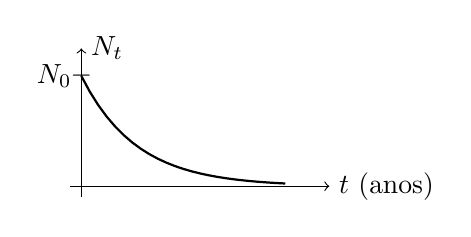
\begin{tikzpicture}
\begin{scope}[scale=0.7]
\pgfmathsetmacro{\n}{2};
\draw[->] (-0.2,0)--(4.5,0) node[right]{$t$ (anos)};
\draw[->] (0,-0.2)--(0,\n+0.5) node[right]{$N_t$};
\draw[thick, domain=0:3.7] plot (\x,{\n*exp(-\x)});
\draw (0,\n) node{$-$} node[left]{$N_0$};
\end{scope}
\end{tikzpicture}\end{bmlimage}
\end{center}
\end{ex}

\begin{exo} Considere \eqref{eq:desintegra}.
\begin{enumerate} 
\item Calcule o tempo de \grasA{meia-vida}\index{tempo de meia-vida} $T$, isto é, o tempo
necessário para a
quantidade de substância ser igual à metade da sua quantidade inicial.
Qual é a quantidade de substância sobrando depois de duas meia-vidas? Quatro? 
Existe um tempo em que a substância toda se desintegrou?
\item Sabendo que o urânio $235$ possui uma taxa de desintegração
$\lambda_U=9.9\cdot 10^{-10}$, calcule o seu tempo de meia-vida.
\end{enumerate}
\begin{sol}
Para ter $N_T=\tfrac{N_0}{2}$, significa que $e^{-\alpha T}=\tfrac12$. Isto é:
$T=\tfrac{\ln 2}{\lambda}$.
Depois de duas meia-vidas, $N_{2T}=N_0e^{-\lambda\tfrac{2 \ln
2}{\lambda}}=\frac{N_0}{4}$ ($>0$: logo, duas meia-vidas não são suficientes
para acabar com a substância!). 
Para quatro, $N_{4T}=\frac{N_0}{16}$. Depois de $k$ meia-vidas,
$N_{kT}=\frac{N_0}{2^k}$:
depois de um número qualquer de meia-vidas, sempre sobre alguma coisa...
Para o uranio $235$, a meia-vida vale $T=\frac{\ln 2}{9.9\cdot 10^{-10}}$, isto
é aproximadamente: $700$ milhões de anos.
\end{sol}
\end{exo}

\begin{exo}
Resolva:
\begin{multicols}{2}
 \begin{enumerate}
  \item\label{iteqln0} $\ln (-x)=2$
  \item\label{iteqln1} $\ln (x^2)=0$
  \item\label{iteqln11} $\ln (x+1)+\tfrac{1}{5}=0$
  \item\label{iteqln2} $\ln (1+x^2)=-\tfrac12$
  \item\label{iteqln3} $e^{x}+e^{-x}=4$
\item\label{iteqln4}$e^{2x-1}<\sqrt{e}$
\item\label{iteqln5}$e^{\tfrac{2x-1}{3x+1}}>\tfrac{1}{e^2}$
\item\label{iteqln6}$\ln(\frac{2x-1}{5x+1})<0$
\item\label{iteqln7} $\ln |x+4|+\ln |x-1|=\ln 6$
\item\label{iteqln8} $(\ln x)^2+\ln x\geq 0$
 \end{enumerate}
\end{multicols}
\vspace{0.01cm}
\begin{sol}
\eqref{iteqln0} $S=\{-e^2\}$
\eqref{iteqln1} $S=\{\pm 1\}$ Obs: aqui, se escrever $\ln(x^2)=2\ln x$, perde-se
a solução negativa! Lembre que $\ln (x^y)=y\ln x$ vale se $x$ é positivo! Então
aqui poderia escrever $\ln(x^2)=\ln (|x|^2)=2\ln |x|$.
\eqref{iteqln11} $S=\{e^{-\tfrac15}-1\}$
\eqref{iteqln2} $S=\varnothing$
\eqref{iteqln3} $S=...$
\eqref{iteqln4} $S=(-\infty,\tfrac34)$
\eqref{iteqln5} $S=(-\infty,-\tfrac13)\cup (-\tfrac18,\infty)$
\eqref{iteqln6} $S=(-\infty,-\tfrac23)\cup (\tfrac12,\infty)$
\eqref{iteqln7} $S=\{-5,-2,-1,2\}$
\eqref{iteqln8} $S=(0,e^{-1}]\cup [1,+\infty)$
\end{sol}
\end{exo}

\begin{exo}
Determine quais das funções abaixo são pares, ímpares, ou nem par e nem
ímpar\index{função! par}.
\begin{multicols}{4}
\begin{enumerate}
\item\label{itparidadelog1} $e^x$
\item\label{itparidadelog2} $\ln x$
\item\label{itparidadelog3} $e^{x^2-x^4}$
\item\label{itparidadelog4} $e^x+e^{-x}$
\item\label{itparidadelog5} $e^x-e^{-x}$
\item\label{itparidadelog6} $\ln (1-|x|+x^2)$
\item\label{itparidadelog7} $\frac{e^{x^2}+e^{|x|}}{x^4+x^6+1}$
\end{enumerate}
\end{multicols}
\vspace{0.01cm}
\begin{sol}
\eqref{itparidadelog1} Nem par nem ímpar.
\eqref{itparidadelog2} Nem par nem ímpar (aqui, tem um problema de domínio: o
domínio do $\ln$ é $(0,\infty)$, então nem faz sentido verificar se 
$\ln (-x)=\ln (x)$).
\eqref{itparidadelog3} Par: $e^{(-x)^2-(-x)^4}=e^{x^2-x^4}$.
\eqref{itparidadelog4} Par.
\eqref{itparidadelog5} Ímpar.
\eqref{itparidadelog6} Par (cuidado com o domínio: $\bR\setminus\{0\}$)
\eqref{itparidadelog7} Par.
\end{sol}
\end{exo}

\begin{exo} 
Esboce o gráfico da função $g(x)\pardef \frac{1}{(x-1)^2}$.
Em seguida, esboce o gráfico da função $f(x)\pardef (\ln \circ g)(x)$ somente a
partir das propriedades do gráfico de $g$ e das propriedades do $\ln$.
\begin{sol}
Sabemos que o gráfico de $\frac{1}{(x-1)^2}$ é obtido transladando o de
$\frac{1}{x^2}$ de uma unidade para direita.
\begin{center}
\begin{bmlimage}\begin{tikzpicture}[scale=0.7]
\draw [ ->] (0,-1)--(0,2) node[left]{$y$};
\draw [ ->] (-3,0)--(4,0) node[right]{$x$};
\pgfmathsetmacro{\a}{3.5}
\pgfmathsetmacro{\e}{0.5}
\draw [thick, domain=-2:1-\e, samples=100] plot (\x,{1/((\x-1)^2)});
\draw [thick, domain=1+\e:4, samples=100] plot (\x,{1/((\x-1)^2)});
%\draw [thick, domain=0.5:\a, samples=100] plot (\x,{\x^{-2}});
%\draw[dotted] (-3,0)--(4,0);
\draw[dotted] (1,-1)--(1,3);
\fill (0,1) circle (0.55mm);
\fill (2,1) circle (0.55mm);
\end{tikzpicture}\end{bmlimage}
\end{center}
Ao tomar o logaritmo de $g(x)$, $f(x)=\ln(g(x))$, é bom ter o gráfico da função
$\ln x$ debaixo dos olhos. 
Quando $x$ é grande (positivo ou negativo),
$g(x)$ é próximo de zero, logo $f(x)$ vai tomar valores grandes e negativos.
Quando $x$ cresce, $g(x)$ cresce até atingir o valor $1$ em $x=0$, logo $f(x)$
cresce até atingir o valor $0$ em $0$. Entre $x=0$ e $x=1$ ($x<1$), $g(x)$
diverge, logo $f(x)$ diverge também.
Entre $x=1$ ($x>1$) e $x=2$, $g(x)$ decresce até atingir o valor $1$ em $x=2$,
logo $f(x)$ decresce até atingir o valor $0$ em $x=2$. 
Para $x>2$, $g(x)$ continua decrescendo, e toma valores que se aproximam de $0$,
logo $f(x)$ se toma valores negativos, e decresce para tomar valores
arbitrariamente grandes negativos.
\begin{center}
\begin{bmlimage}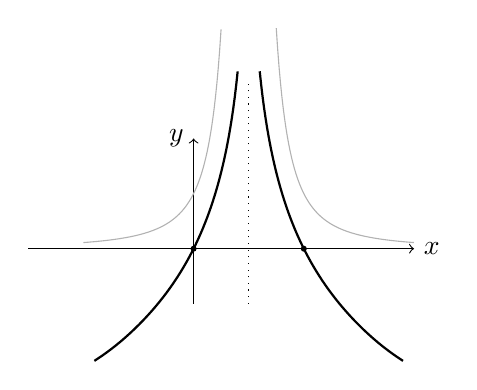
\begin{tikzpicture}[scale=0.7]
\draw [ ->] (0,-1)--(0,2) node[left]{$y$};
\draw [ ->] (-3,0)--(4,0) node[right]{$x$};
\pgfmathsetmacro{\a}{3.5}
\pgfmathsetmacro{\e}{0.5}
\draw [color=gray!60, domain=-2:1-\e, samples=100] plot (\x,{1/((\x-1)^2)});
\draw [color=gray!60, domain=1+\e:4, samples=100] plot (\x,{1/((\x-1)^2)});
\pgfmathsetmacro{\e}{0.2}
\draw [thick, domain=-1.8:1-\e, samples=100] plot (\x,{ln(1/((\x-1)^2))});
\draw [thick, domain=1+\e:3.8, samples=100] plot (\x,{ln(1/((\x-1)^2))});
\draw[dotted] (1,-1)--(1,3);
\fill (0,0) circle (0.55mm);
\fill (2,0) circle (0.55mm);
\end{tikzpicture}\end{bmlimage}
\end{center}
Observe que é também possível observar que $f(x)=-2\ln|x-1|$, e obter o seu
gráfico a partir do gráfico da função $\ln |x|$!

\end{sol}
\end{exo}

\begin{exo}
Determine o conjunto imagem da função $f(x)\pardef
\frac{e^{x}}{e^{x}+1}$.
\begin{sol}
Lembramos que $y\in \bR$ pertence ao conjunto imagem de $f$ se e somente
se existe um $x$ (no domínio de $f$) tal que $f(x)=y$.
Ora $\frac{e^{x}}{e^{x}+1}=y$ implica $e^x=\frac{y}{1-y}$. Para ter uma
solução, é necessário ter $\frac{y}{1-y}>0$. É fácil ver que
$\frac{y}{1-y}>0$ se e somente se $y\in (0,1)$. Logo, 
$\mathrm{Im}(f)=(0,1)$. 
\end{sol}
\end{exo}

\section[Funções hiperbólicas]{Funções trigonométricas hiperbólicas}\label{Sec:FuncTrigHiperb}
\index{funções trigonométricas! hiperbólicas}
A exponencial na base $e$ 
permite definir três funções fundamentais chamadas respectivamente 
\grasA{seno
hiperbólico}\index{seno! hiperbólico}, \grasA{cosseno 
hiperbólico}\index{cosseno!
hiperbólico} e \grasA{tangente hiperbólica}\index{tangente! hiperbólica}:
\eq{
\boxed{
\senh x\pardef \frac{e^x-e^{-x}}{2}\,,\quad 
\cosh x\pardef \frac{e^x+e^{-x}}{2}\,,\quad 
\tanh x\pardef
\frac{e^x-e^{-x}}{e^x+e^{-x}}\,.}
}

Para entender a origem da mistura de terminologia (nada óbvia a priori!) 
usada para definir essas funções, ``trigonometria'' e 
``hipérbole''\index{hipérbole}, o leitor
interessado poderá consultar o texto da Professora Sônia Pinto de
Carvalho~\footnote{\texttt{www.mat.ufmg.br/$\sim$sonia/pubensino.htm}}.
Estudaremos mais a fundo as propriedades dessas funções nos próximos 
capítulos; por enquanto faremos somente alguns comentários.\\

Observe primeiro que
$$\tanh x=\frac{\senh x}{\cosh x}\,, $$
Também,
$$
\Bigl( \frac{e^x+e^{-x}}{2}\Bigr)^2-\Bigl(
\frac{e^x-e^{-x}}{2}\Bigr)^2=\frac{e^{2x}+2+e^{-2x}}{4}-
\frac{e^{2x}-2+e^{-2x}}{4}=1\,,
$$
portanto vale a seguinte identidade,
\eq{\label{eqtrigohiperb2}\cosh^2x-\senh^2x=1\,,}
que tem uma semelhança com \eqref{eqtrigo2}: $\cos^2x +\sen^2x=1$. 

\begin{exo}
Mostre que $\cosh x$ é uma função par, e que $\senh x$ e $\tanh x$ são ímpares.
\begin{sol}
Por exemplo, $\senh (-x)=\frac{e^{(-x)}-e^{-(-x)}}{2}=\frac{e^{-x}-e^{x}}{2}
=-\frac{e^{x}-e^{-x}}{2}=-\senh (x).$
\end{sol}
\end{exo}

Os gráficos das funções hiperbólicas serão estudados em detalhes nos próximos
capítulos. Mencionaremos somente o seguinte fato:
o gráfico da 
função $\cosh x$ aparece a cada vez que uma corda\index{corda} é pendurada entre 
dois pontos $A$ e $B$:
\begin{center}
\begin{bmlimage}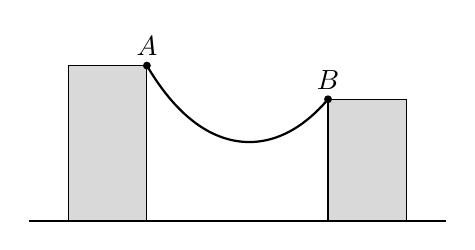
\begin{tikzpicture}
\pgfmathsetmacro{\a}{-1.3};
\pgfmathsetmacro{\b}{1};
\coordinate (A) at (\a,{(exp(\a)+exp(-1*\a))/2});
\coordinate (B) at (\b,{(exp(\b)+exp(-1*\b))/2});
\fill[color=gray!30] (\a-1,0) rectangle (A);
\fill[color=gray!30] (\b+1,0) rectangle (B);
\draw (\a-1,0) rectangle (A);
\draw (\b+1,0) rectangle (B);
\draw [thick, domain=\a:\b, samples=100] plot (\x,{(exp(\x)+exp(-1*\x))/2});
%\coordinate (pB) at (\b,0);
\fill (A) circle (0.50mm);
\fill (B) circle (0.50mm);
\draw (A) node[above]{$A$};
\draw (B) node[above]{$B$};
\draw[thick] (\a-1.5,0)--(\b+1.5,0);
%\draw[thick] (\b,0)--(B);
\end{tikzpicture}\end{bmlimage}
\end{center}



%%%NAO USADO:
%\section{Diagramas $\log-\log$}


